\chapter{Experimentos}\label{cap.experimentos}
\hspace{1cm} En este capítulo se describen los experimentos realizados para validar el prototipo final, para comprobar el correcto funcionamiento del algoritmo completo y llegar a una solución final tras depurar mientras se desarrollaba. Para ello se ha dividido el capítulo en tres partes a analizar: la primera parte, se ha comprobado la calidad de autolocalización, es decir, se ha realizado una ruta teleoperada para ver los errores de posición de la aplicación; la segunda parte, se ha evaluado la calidad del controlador, es decir, el error que comente el piloto al realizar una ruta predefinida y por último, se ha validado el funcionamiento de la aplicación final con todos los componentes a la vez.

\hspace{1cm} Dada la complejidad de los experimentos, se han llevado a cabo dentro del entorno de simulación Gazebo. El plugin para la simulación del comportamiento del drone, así como el modelo necesario para la renderización del vehículo y sus sensores están incluidos en JdeRobot. Pero para realizar correctamente los diferentes experimentos se han creado una serie de mundos en 3D, los cuales cuentan con espacios abiertos, espacios cerrados, balizas arlequinadas y balizas AprilTags con sus correspondientes texturas. Los mundos creados se han integrado en el repositorio oficial de JdeRobot bajo los nombres de \textit{ArDrone1}, \textit{ArDrone2} y \textit{ArDrone3}.

\hspace{1cm} En la Figura \ref{fig:Mundo Gazebo.} se puede observar el mundo ArDrones1, que fue el primero que creamos y el más representativo ya que se puede observar una posible aplicación de reconocimiento de un casa mediante el dron completamente automatizado. Cuenta con las balizas arlequinadas de despegue (verde-naranja) y aterrizaje (verda-azul), con balizas 23 AprilTags para la autolocalización que rodean una casa a la cual el drone tiene que darle una vuelta completa.

\begin{figure}[H]
	\begin{center}
		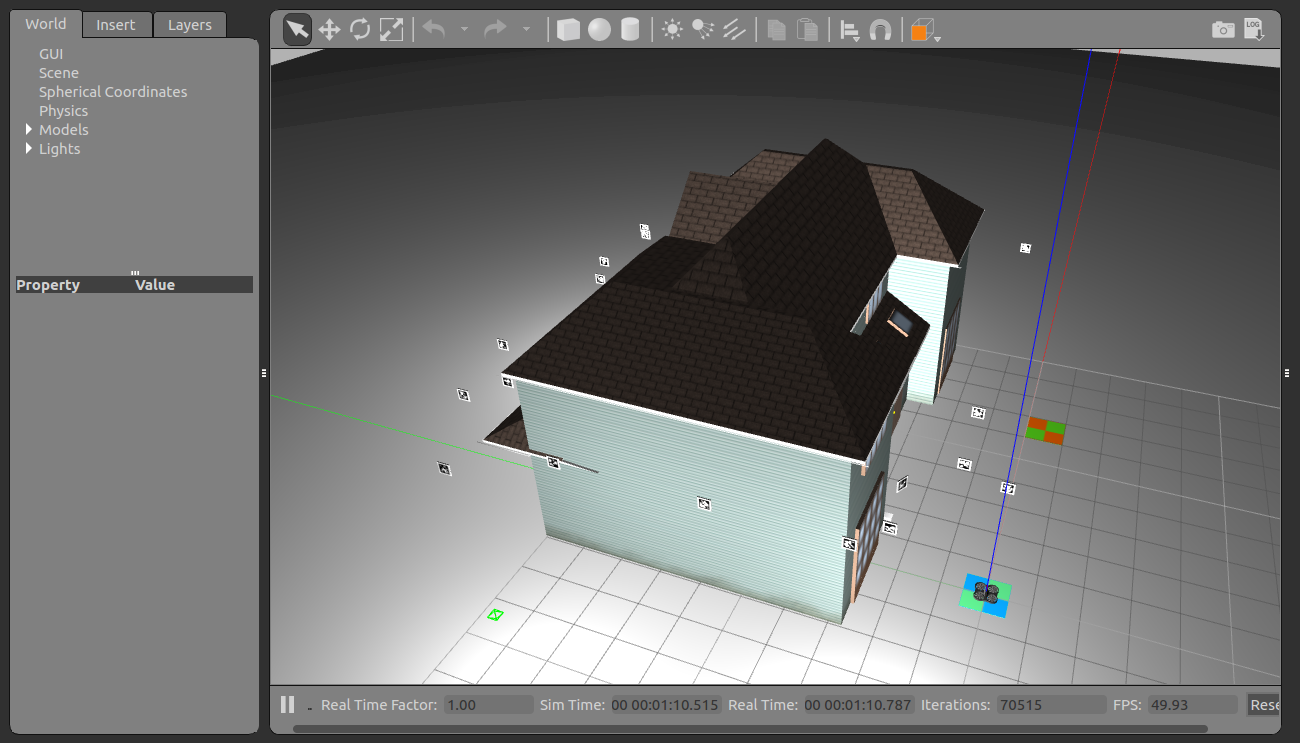
\includegraphics[width=1\textwidth]{imag/IMG28.png}
				\caption{Mundo Gazebo ArDones1.}
		\label{fig:Mundo Gazebo.}	
	\end{center}
\end{figure}

\hspace{1cm} Tanto para el cálculo de trayectorias, como para el cálculo de errores de distancia y de tiempos de ruta, se ha hecho uso del programa Matlab, el cual nos ha facilitado todos los procesos de cálculo.

\section{Pruebas unitarias de autolocalización}
\hspace{1cm} Para evaluar el comportamiento del componente \texttt{Slam VisualMarkers} que se encarga de la autolocalización del drone, se aisló completamente de la parte de pilotaje. Para ello lo que se hizo fue teledirigir a mano el drone dentro de un mundo de balizas el cual permitiese al componente ver al menos una baliza AprilTag en todo momento de la ruta. Una vez terminada la ruta se comparó la secuencia de posiciones reales entregada por el simulador $P_{0}$ con la secuencia de posiciones estimadas por el componente $P_{A} $. Dado que ambas entregan tanto posición (x y z) como dirección (Pitch Roll Yaw) se realizó un cálculo de error de posición mediante la distancia euclídea: 
\[ E_{p} = \sqrt{(P_{Ax}-P_{0x})^{2}+(P_{Ay}-P_{0y})^{2}+(P_{Az}-P_{0z})^{2}}\]
y lo que hemos definido como el \textit{error angular}:    
\[ E_{a} = \sqrt{(P_{AP}-P_{0P})^{2}+(P_{AR}-P_{0R})^{2}+(P_{AY}-P_{0Y})^{2}}\]

\begin{figure}[H]
	\begin{center}
		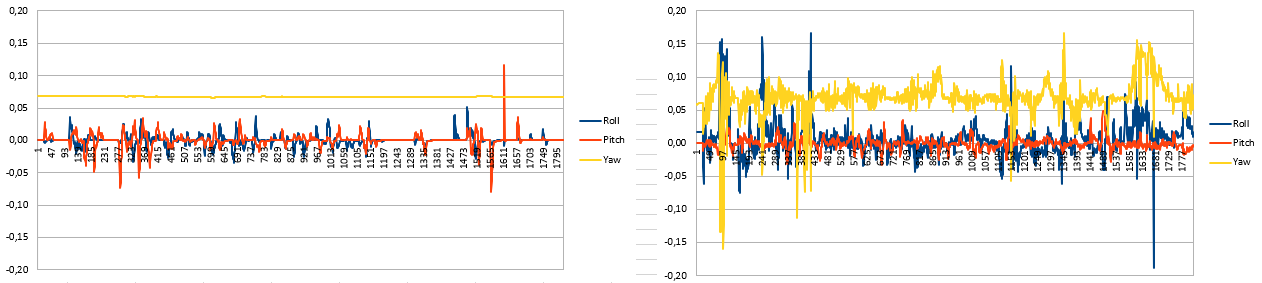
\includegraphics[width=1\textwidth]{imag/IMG90.PNG}
				\caption{Diferencia angular entre lo real y VisualMarkers}
		\label{fig:Error angular.}	
	\end{center}
\end{figure}

\begin{figure}[H]
	\begin{center}
		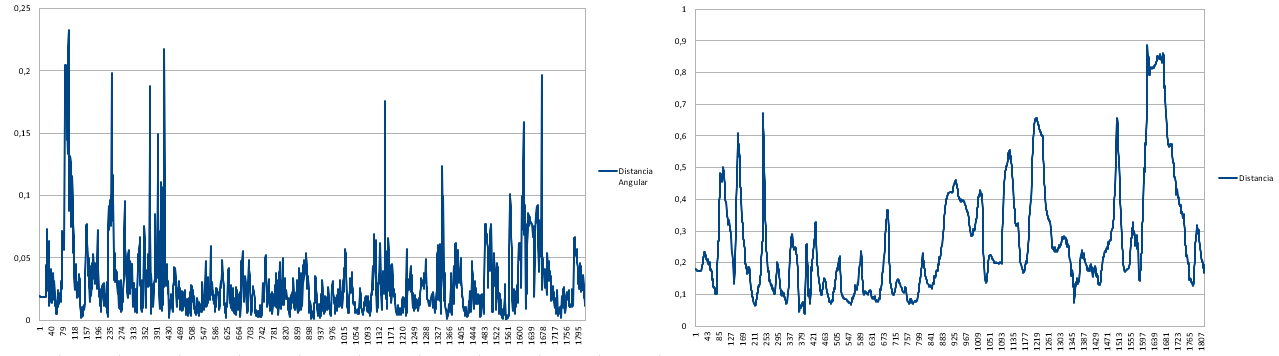
\includegraphics[width=1\textwidth]{imag/IMG91.PNG}
				\caption{Cálculo de errores de distancia y de ángulos}
		\label{fig:Error de distancia y de giro.}	
	\end{center}
\end{figure}

\hspace{1cm} Con la aplicación de las fórmulas anteriores se obtuvieron las gráficas de la figura \ref{fig:Error de distancia y de giro.}. En las gráficas superiores se ve la diferencia entre los tres ángulos pitch, roll y yaw del drone real (izquierda) con los calculados por el componente Slam VisualMarkers (derecha). Comparando visualmente las gráficas parece que el error sea elevado pero una vez analizados numéricamente los datos y calculando los errores con la fórmula anterior y representándolos en la gráfica izquierda de la Fig \ref{fig:Error de distancia y de giro.} se ve como el error angular medio es de 0.0293rad lo que equivale a 1.679 grados, que es un error muy pequeño, el error angular máximo es de 0.2329rad que son 13.344 grados. Por último. la gráfica derecha de la Fig \ref{fig:Error de distancia y de giro.} nos muestra los errores de distancia euclídea entre la ruta realizada realmente con la posición que se calculaba con Slam-VisualMarkers, esta nos da que el error medio de distancia euclídea es de 0.2651m y el error máximo de distancia euclídea es de 0.8856m. Con el cálculo de estos números y teniendo en cuenta que los errores máximos se producen cuando el drone sólo ve una baliza y esta está alejada son cifras bastante razonables.

\begin{figure}[H]
	\begin{center}
		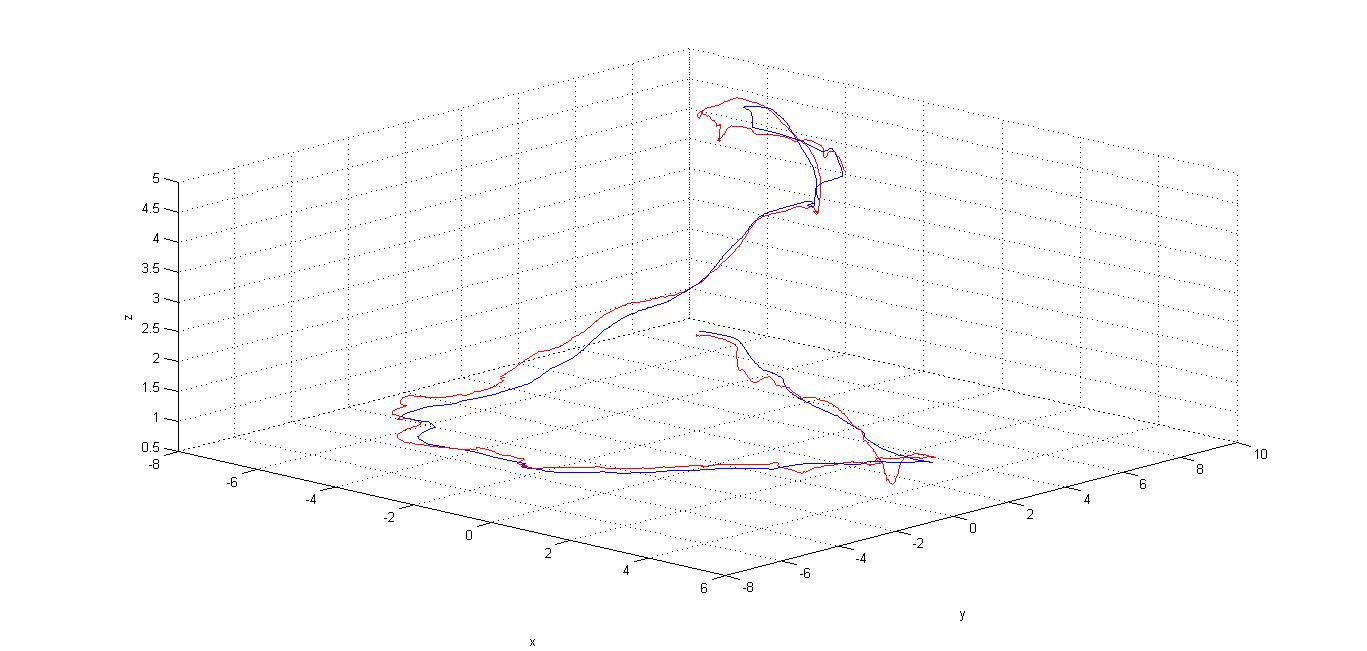
\includegraphics[width=1\textwidth]{imag/IMG48.jpg}
				\caption{Cálculo de posición de Slam-VisualMarkers}
		\label{fig:Comparativa Slam-Visualmarkers.}	
	\end{center}
\end{figure}

\hspace{1cm} Una vez realizados los cálculos del error se comprobó como cuando el componente pierde de vista las AprilTags los errores de posicionamiento aumentan considerablemente como se puede observar en la Figura \ref{fig:Comparativa Slam-Visualmarkers.}, en la cual tenemos la ruta realizada en azul y la ruta estimada por el componente en rojo. Para evitar esto se habló con el desarrollador de Slam VisualMarkers y se añadió más información a su interfaz de salida en ROS de modo que ya indicaba el número de balizas que se estaban viendo. Esta caracterización experimental de la autolocalización permitió acotar los márgenes de error con los que tenía que lidiar el nodo de pilotaje y permitió mejorar la navegación autónoma contemplando la situación en la que el drone se perdía. Con esto se pudo crear un nuevo comportamiento que permite que cuando el drone no esté viendo ninguna baliza no siga la ruta, sino que gire sobre sí mismo realizando círculos, cada vez mayores, sobre el último punto donde veía alguna baliza, para así poder volver a encontrarla y posicionarse correctamente. Esto ayudó a que el drone no se perdiese de la ruta y siguiese moviéndose cuando no encontraba ninguna baliza, ya que ahora si da tres vueltas y seguía sin encontrar ninguna baliza, el drone aterriza. Con esta nueva función mejoramos la integridad de la aplicación de navegación autónoma y nos aseguramos de que el cuadricóptero no se aleje excesivamente de la ruta definida, preparándolo para los experimentos reales.

\section{Pruebas unitarias de pilotaje}
\hspace{1cm} A diferencia de las pruebas anteriores, en estas pruebas se suministraba al piloto la posición verdadera del drone en todo momento, extraida del simulador. Así, los errores entre la ruta deseada y la realmente conseguida son exclusivamente achacables al pilotaje, no a la autolocalización. 

\subsection{Pilotaje por puntos de paso}
\hspace{1cm} El primer piloto desarrollado se encargaba de seguir únicamente puntos de paso, es decir tan solo variaría la velocidad lineal del drone. Los primeros experimentos mostraban como el piloto se acercaba correctamente al punto, pero en la aproximación final no lograba alcanzarlo, por lo que se tuvieron que realizar varias correcciones, tanto de velocidades máximas en los ejes x e y, como de variaciones de velocidad según la cercanía al siguiente punto de paso. Una vez conseguido esto se volvieron a ajustar los parámetros de velocidades máximas, esta vez en los tres ejes para conseguir que el error en una ruta por puntos nunca superase los 10cm. Para ello se tuvo que sacrificar la velocidad máxima cuando el drone se acercaba al siguiente punto de paso, pero aun así, la velocidad media del drone continuaba siendo el 0.82 de la máxima.

\hspace{1cm} En la Figura \ref{fig:Error asociado al pilotaje.} se puede ver una ruta por puntos compleja (en verde) y cómo ajustando la velocidad cercana a los puntos, la ruta final del drone es más exacta (rojo) que permitiéndole una velocidad máxima mayor (azul). Con todos estos ajustes y alternativas probadas, al final se ofrece un piloto que se puede configurar para que realice la ruta con mayor rapidez o con una mayor exactitud, recalcando que el error introducido por el pilotaje es aceptable, que consigue pasar por todos los puntos de paso especificados con un error por debajo de 0.02m.

\begin{figure}[H]
	\begin{center}
		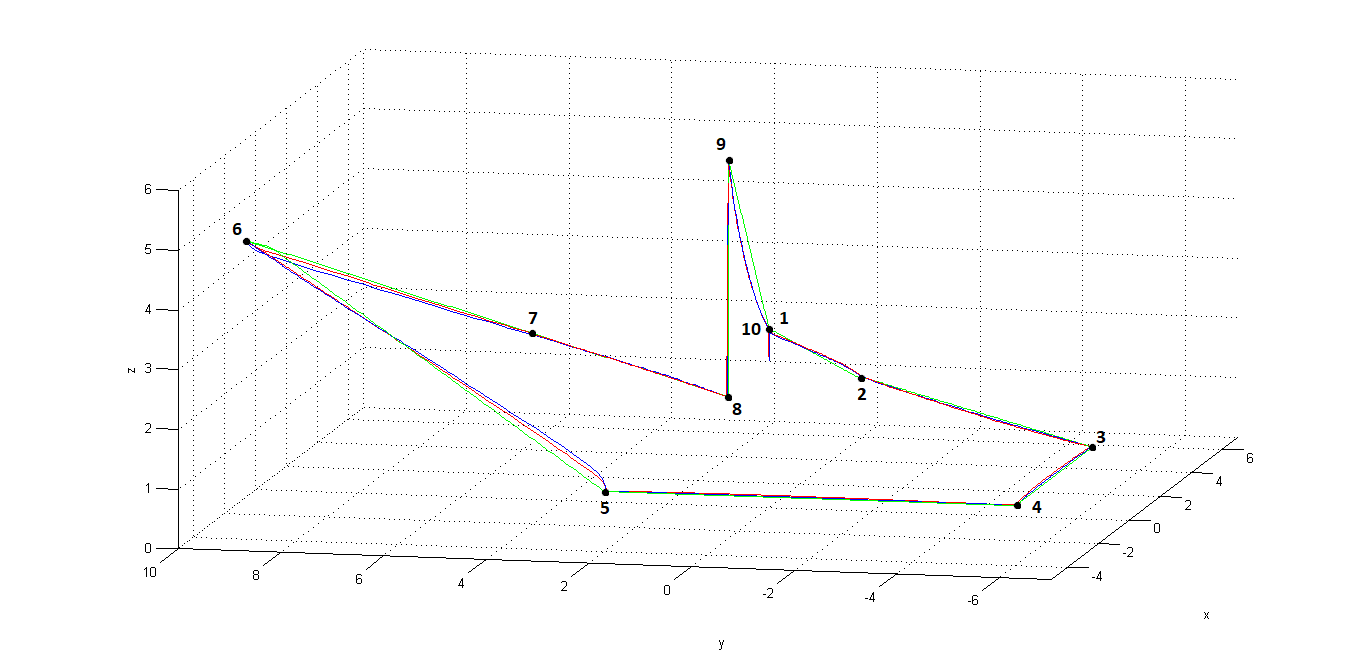
\includegraphics[width=1.0\textwidth]{imag/IMG47.png}
				\caption{Seguimiento de ruta por puntos de paso en 3D.}
		\label{fig:Error asociado al pilotaje.}	
	\end{center}
\end{figure}

\subsection{Pilotaje por puntos de paso}
\hspace{1cm} Después de validar el correcto funcionamiento del piloto por puntos se observó que este piloto sólo sería valido para ciertas situaciones concretas de espacios abiertos, por lo que se desarrolló un segundo piloto, el piloto por trayectorias continuas que permite un control más fino de las posiciones del drone. Éste es más complejo ya que tiene variaciones de velocidad lineal y angular (en el ángulo de \textit{yaw}), al introducir giros el sistema presenta comportamientos inestables. Para solucionar este comportamiento se realizó un estudio de relaciones de velocidades y se observó que el rango de velocidades para el funcionamiento estable del sistema de navegación era de [0.3-3.2]m/s. Del mismo modo, los valores de ganancia de giro debían estar comprendidos entre el rango [0.14-0.36]. Esta ganancia de giro era muy importante ya que valores muy altos significaban comportamientos inestables y valores muy bajos no permitían ajustar el giro de forma correcta. 

\hspace{1cm} A continuación se muestran diferentes ejemplos de rutas sencillas y complejas, en los cuales se ha comparado con un piloto anterior, el del PFC de Manuel Zafra \cite{ManuelZafra}, de trayectorias para observar la mejora conseguida tanto reduciendo los errores de distancias a la ruta como acortando el tiempo de realización de rutas.

\hspace{1cm} Empezando con rutas sencillas, en la Figura \ref{fig:Ruta sencilla en trayectoria.} se distinguen: la trayectoria deseada (verde), que es la que se introduce al programa; la trayectoria que realiza el piloto antiguo (azul); y por último, la trayectoria que realiza nuestro piloto (rojo).

\begin{figure}[H]
	\begin{center}
		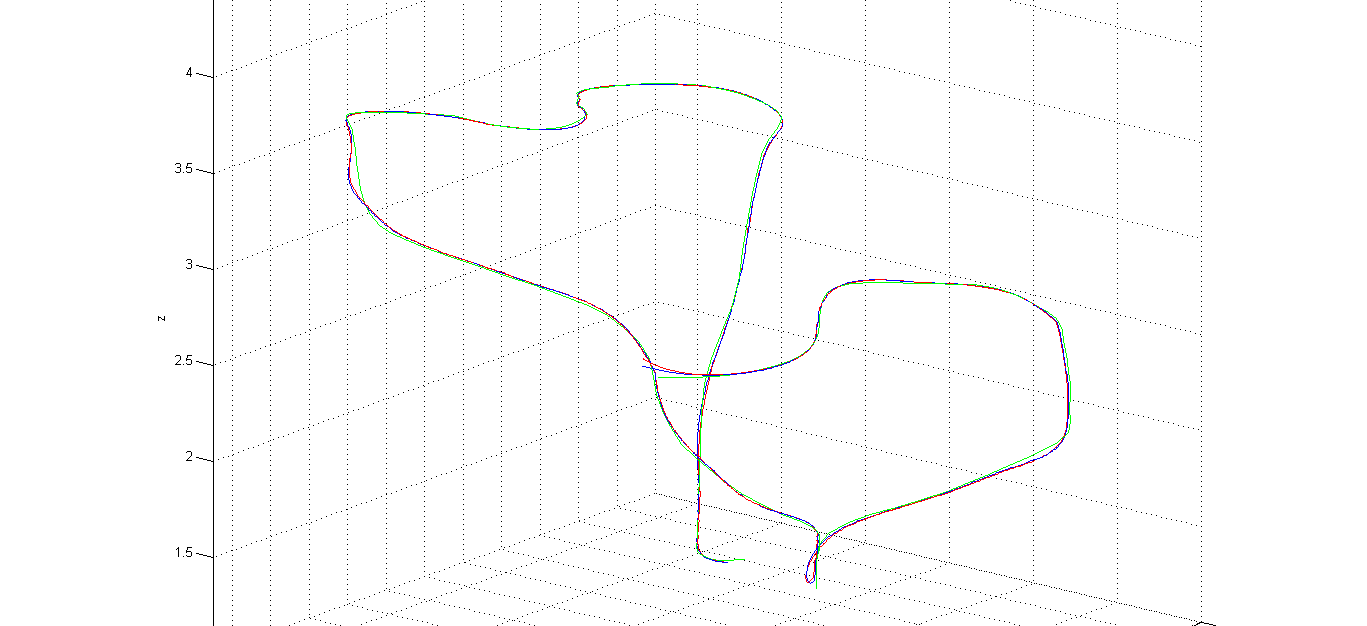
\includegraphics[width=1.0\textwidth]{imag/IMG40.png}
				\caption{Ruta sencilla en el pilotaje por trayectorias.}
		\label{fig:Ruta sencilla en trayectoria.}	
	\end{center}
\end{figure}

\hspace{1cm} En la imagen \ref{fig:Ruta sencilla en trayectoria.} se puede observar cómo ambos pilotos son muy exactos a la hora de realizar las trayectorias deseadas suaves, que no cuentan con cambios de dirección muy bruscos ni con curvas muy cerradas, sobre todo en las partes rectas de las mismas donde se ve como el ajuste es prácticamente perfecto.

\begin{figure}[H]
 \centering
  \subfloat[Piloto Antiguo]{
   \label{f:Piloto Antiguo}
    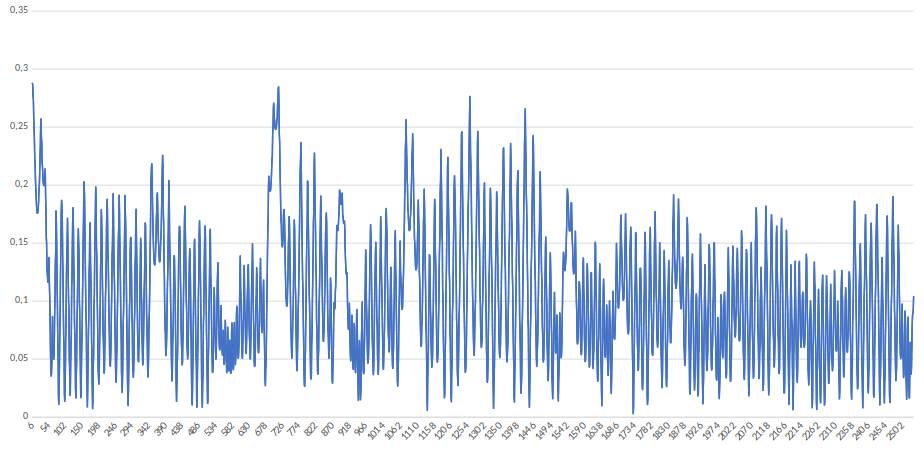
\includegraphics[width=0.5\textwidth]{imag/IMG46.png}}
  \subfloat[Piloto Nuevo]{
   \label{f:Piloto Nuevo}
    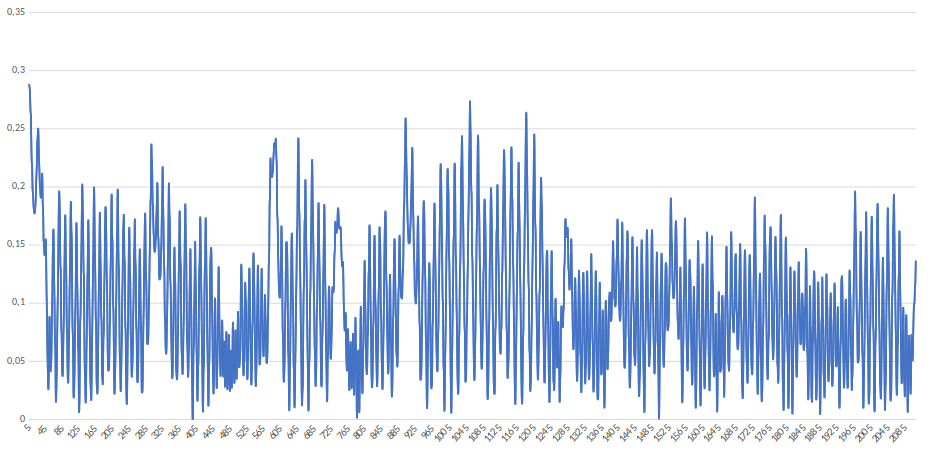
\includegraphics[width=0.5\textwidth]{imag/IMG45.png}} 
 \caption{Comparación del error entre ambos pilotos en ruta sencilla.}
 \label{f:Comparativa del error sencilla.}
\end{figure} 
 
\hspace{1cm} En las gráficas \ref{f:Comparativa del error sencilla.} donde calculando el error obtenemos que el error medio de distancia en nuestro piloto es de 0.1023m con un error máximo en ruta de 0.276m en cambio el piloto antiguo tiene un error medio de 0.1026m y un error máximo de 0.285m. Este error no refleja una diferenciación significativa en cuanto al piloto nuevo y al piloto antiguo en rutas sencillas, en error espacial. Pero sí hay una notable diferencia si nos centramos en el tiempo en que realizan la ruta el piloto nuevo tarda 188.72 segundos mientras que el antiguo utilizaba 253.35 segundos lo que supone una reducción del 25,51\% del tiempo en vuelo, algo muy importante debido a la corta autonomía de los drones.

\begin{figure}[H]
	\begin{center}
		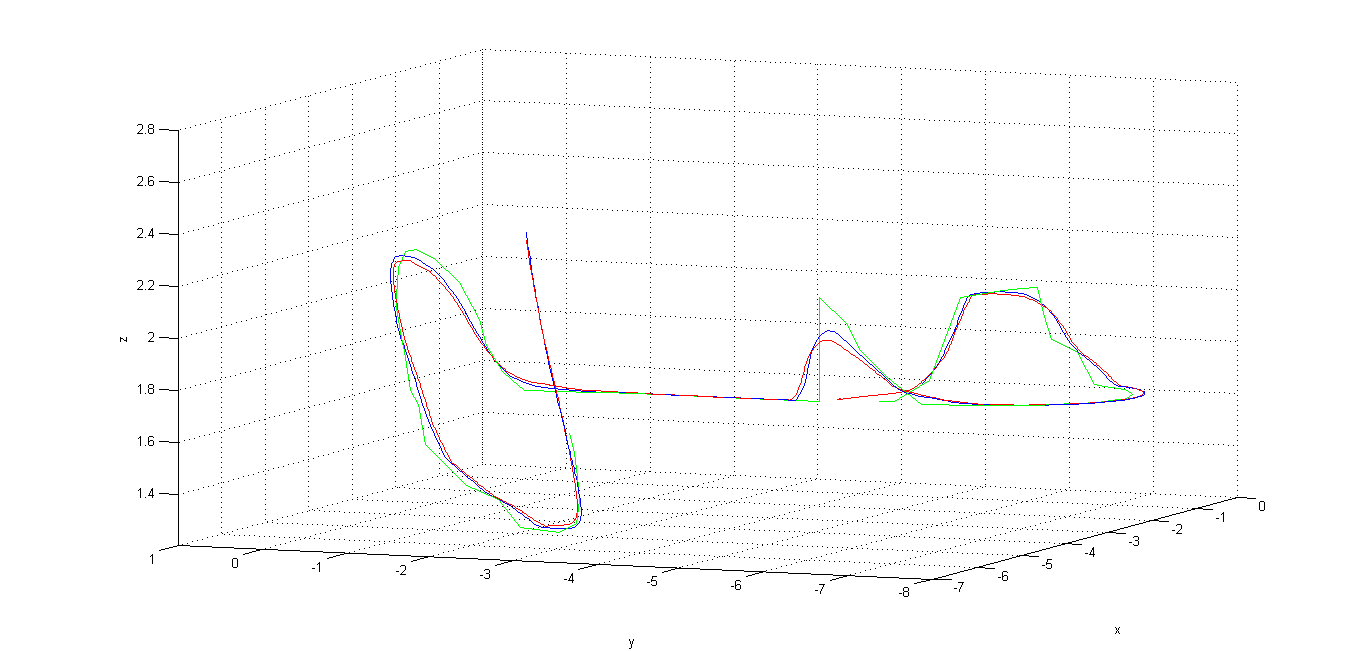
\includegraphics[width=1\textwidth]{imag/IMG41.png}
				\caption{Ruta compleja en el pilotaje por trayectorias.}
		\label{fig:Ruta compleja en trayectoria.}	
	\end{center}
\end{figure}

\begin{figure}[H]
 \centering
  \subfloat[Piloto Antiguo]{
   \label{f:Piloto Antiguo}
    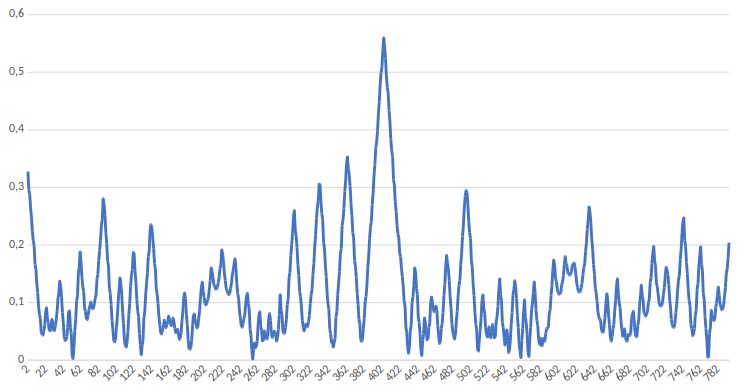
\includegraphics[width=0.5\textwidth]{imag/IMG39.png}}
  \subfloat[Piloto Nuevo]{
   \label{f:Piloto Nuevo}
    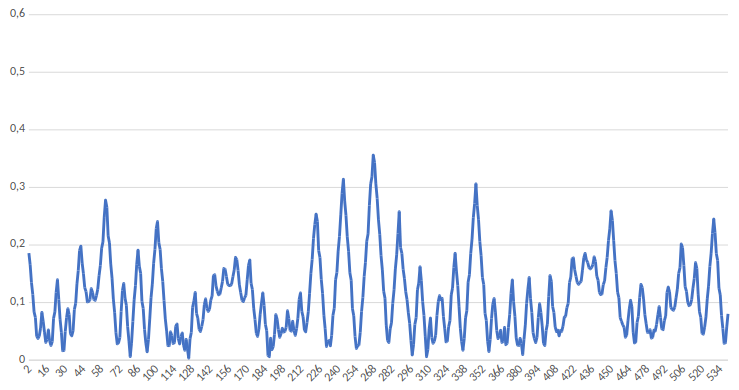
\includegraphics[width=0.5\textwidth]{imag/IMG38.png}} 
 \caption{Comparación del error entre ambos pilotos en ruta compleja.}
 \label{f:Comparativa del error compleja.}
\end{figure} 

\hspace{1cm} En cuanto a rutas complejas, para observar mejor el error en distancia, pedimos a los pilotos a una trayectoria con curvas mucho más pronunciadas y con cambios de altitud bruscos. Esta trayectoria se puede observar en la imagen \ref{fig:Ruta compleja en trayectoria.} donde tenemos la trayectoria deseada en verde, el piloto nuevo en azul y el piloto antiguo en rojo. En esta imagen se ve con mayor claridad cómo el piloto nuevo se ajusta mucho más a la ruta deseada. Estas mejores prestaciones se corroboran con los datos de las gráficas de la Figura \ref{f:Comparativa del error compleja.}, en los cuales el error medio del piloto nuevo es de 0.106m y el error máximo es de 0.356m mientras que el error medio del piloto antiguo es de 0.119m con un error máximo de 0.559m. A su vez el nuevo piloto tarda 59.85 segundos en realizar la ruta mientras que el antiguo lo hace en 84.82 segundos reduciendo en este caso el tiempo de ruta en un 29.44\% por lo que en rutas complejas el nuevo piloto se desenvuelve mejor que el antiguo en todos los aspectos.

\section{Pruebas integrales del sistema}
\hspace{1cm} Una vez conseguido que los componentes por separado funcionasen correctamente, se integraron ambos componentes conjuntamente y se realizaron las pruebas finales del sistema. Con ellas se valida experimentalmente la aplicación completa de navegación desarrollada. Pese a la complejidad de unir los dos componentes ya que cada uno utilizaba unas velocidades máximas del drone y unos datos diferentes de posicionamiento, cuando se consiguió combinar y al haber realizado las pruebas por separado con buenos resultados, se esperaba que al unirlos los resultados siguiesen siendo óptimos. El buen funcionamiento del sistema se corroboró con los experimentos tanto de la ruta por puntos de paso (en la Figura \ref{fig:Prueba integral de ruta por puntos.}) donde tenemos en verde la ruta deseada, en rojo la posición estimada y en azul la ruta realizada, como de la ruta por trayectorias continuas (en la Figura \ref{fig:Prueba integral de ruta por trayectoria.}). En ambos se ve como el drone seguía la ruta de forma estable y con un margen de error prácticamente nulo, siempre y cuando estén a la vista del vehículo aéreo las balizas AprilTags para su autolocalización. 

\begin{figure}[H]
	\begin{center}
		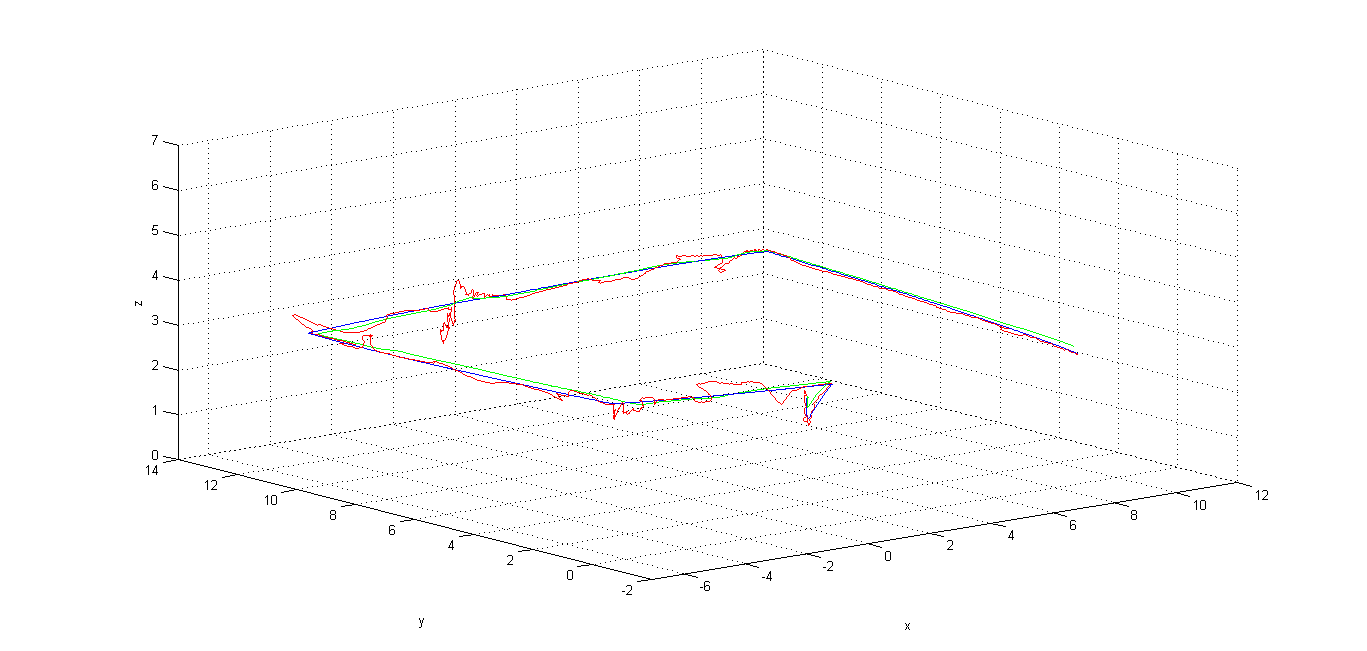
\includegraphics[width=1\textwidth]{imag/IMG42.png}
				\caption{Prueba integral de ruta por puntos.}
		\label{fig:Prueba integral de ruta por puntos.}	
	\end{center}
\end{figure}

\begin{figure}[H]
	\begin{center}
		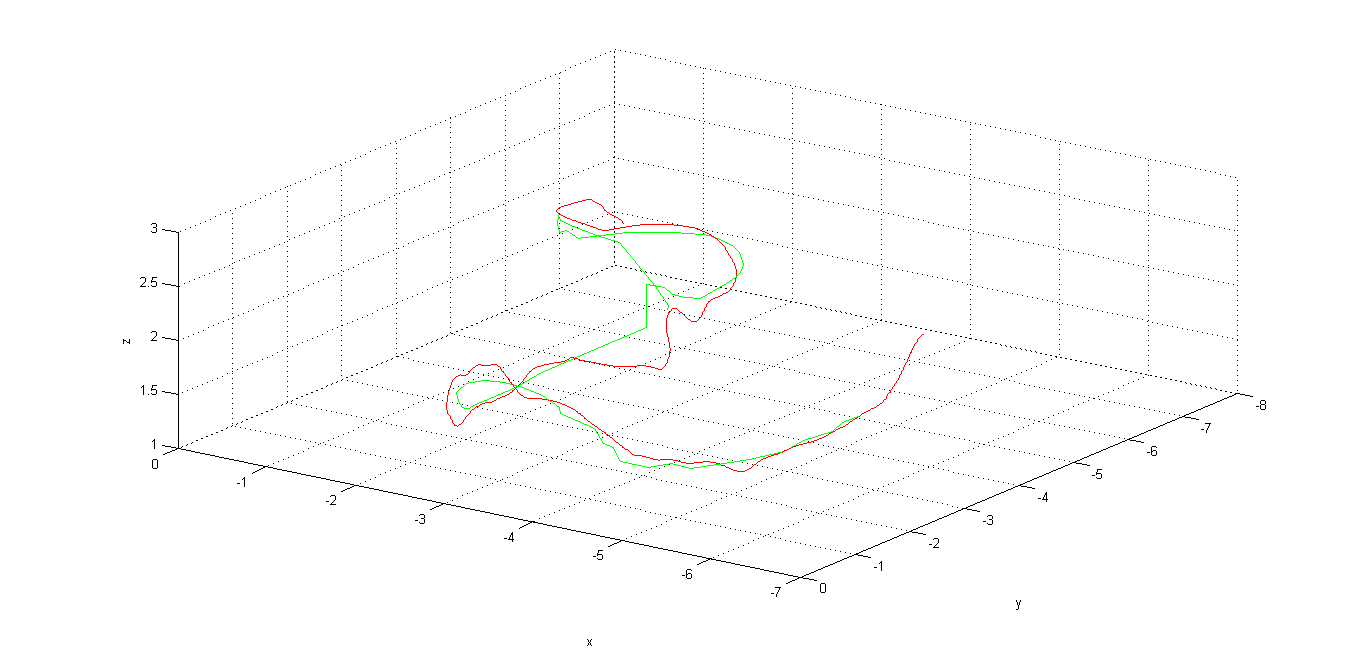
\includegraphics[width=1\textwidth]{imag/IMG43.png}
				\caption{Prueba integral de ruta por trayectoria.}
		\label{fig:Prueba integral de ruta por trayectoria.}	
	\end{center}
\end{figure}

\hspace{1cm} Para el experimento de la navegación integral por trayectoria continua decidimos utilizar una ruta compleja con curvas cerradas y saltos de altura, y así comprobar la integridad y el error de la aplicación para cualquier situación puesto que ése es el escenario de navegación más complejo. En la imagen \ref{fig:Prueba integral de ruta por trayectoria.} se observa la ruta deseada en verde y la ruta realizada en rojo. A primera vista no se aprecian errores demasiado elevados, por lo que analizamos con más detalle lo datos de error de distancia en la Figura \ref{fig:Error de distancia final.}. De este análisis extraemos que el error medio de distancia en esa ruta compleja fue de 0.128m con un error máximo de 0.563m. Este alto error máximo, que es puntual, se debe a que el reconocimiento de las balizas no se puede realizar a velocidades elevadas, el tiempo de ruta fue de 109.5 segundos.

\begin{figure}[H]
	\begin{center}
		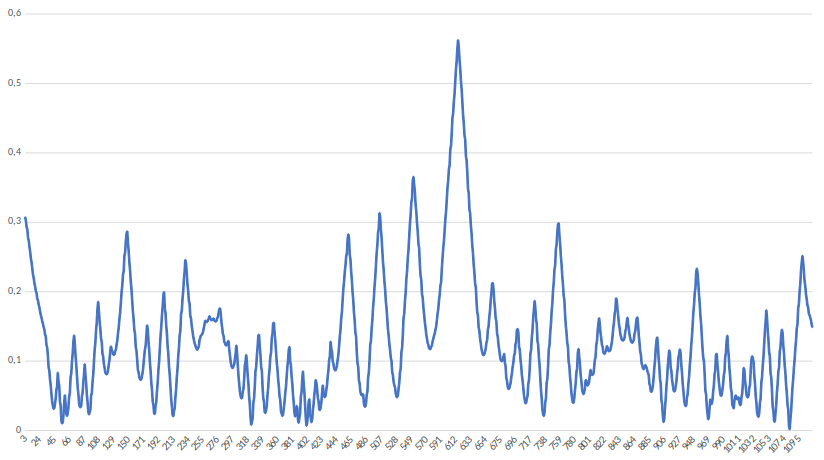
\includegraphics[width=1\textwidth]{imag/IMG44.png}
				\caption{Error de distancia a la ruta deseada en la prueba integral del sistema}
		\label{fig:Error de distancia final.}	
	\end{center}
\end{figure}


\hspace{1cm} Este error entre la trayectoria ideal y la trayectoria conseguida incluye y acumula dos fuentes de errores independientes: los errores debidos a una mala autolocalización y los errores debidos a un mal pilotaje de los motores del drones. Es interesante destacar que este error medido experimentalmente es similar al que se obtenía cuando se alimenta al pilotaje con las posición 3D perfecta del drone (figura \ref{fig:Prueba integral de ruta por trayectoria.}).

\hspace{1cm} Por último, anotar que el piloto desarrollado cuenta con un margen de error de 15cm, lo que permite al vehículo realizar maniobras más amplias para evitar giros abruptos y así conseguir estabilidad durante toda la ruta. 

\hspace{1cm} También se ha enriquecido el controlador con dos funcionalidades que lo preparan para el mundo real. Primero, cuando un punto no lo puede alcanzar correctamente por una limitación en sus movimientos aterrice y no se quede infinitamente dando vueltas sobre este punto sin probabilidad de éxito. Segundo, una nueva función basada en el nuevo \texttt{Slam VisualMarkers} de ROS utilizando el número de balizas observadas en imagen. En el momento que está 2 segundos sin ver ninguna baliza AprilTag el drone interrumpe su intento de seguir la ruta, ya que no está recibiendo una localización real, y gira en círculos cada vez mayores en torno al último punto para así encontrar la baliza anterior y poder volver a localizarse. Si consigue observarla continuar siguiendo la ruta, si no, aterrizará para evitar que tenga una autolocalización errónea y se pierda en su intento de seguir la ruta deseada.